%This is a experiment example of ZhengXiaoyang's experiment report template

\documentclass[UTF8]{ctexart}
 
\usepackage{amsmath}
\usepackage{cases}
\usepackage{cite}
\usepackage{xeCJK}
\usepackage{graphicx}
\usepackage[margin=1in]{geometry}
\geometry{a4paper}
\usepackage{fancyhdr}
\pagestyle{fancy}
\fancyhf{}

\graphicspath{{picture/}}


\title{利用霍尔传感器测量磁场}
\graphicspath{{picture/}}


\title{利用霍尔传感器测量磁场}
\author{郑晓旸}
\date{\today}
\pagenumbering{arabic}

\begin{document}
%这里是文件的开头
\fancyhead[L]{郑晓旸}
\fancyhead[C]{磁场测量}
\fancyfoot[C]{\thepage}

\maketitle
\tableofcontents
\newpage

\section{实验目的}
    \begin{enumerate}
        \item 了解霍尔传感器的工作原理以及标定方法
        \item 研究亥姆霍兹线圈的磁场分布规律 
        \item 研究测量磁介质对磁场的分布的影响
    \end{enumerate}

\section{实验仪器}
    \begin{enumerate}
        \item 多种磁场传感器及适配模块
        \item 电源
        \item 换向开关
        \item 亥姆霍兹线圈
        \item 导轨和支架
        \item 多功能物理测试仪
        \item 铁球
    \end{enumerate}

    \section{实验原理}

    \subsection{霍尔效应}
    
    霍尔效应是载流子在磁场中受到洛伦兹力而发生偏转,在材料两侧积累电荷从而形成霍尔电压的现象。如图\ref{fig:hall_effect}所示,设材料中载流子电荷量为 $q$,浓度为 $n$,在电流 $I_S$ 作用下沿 $x$ 方向运动,平均速度为 $v$。施加垂直磁场 $\vec{B}=(0,0,B)$ 后,载流子在洛伦兹力 $\vec{F}_L=q\vec{v}\times\vec{B}$ 作用下沿 $y$ 方向偏转,在两侧形成净电荷,产生横向电场 $\vec{E}=(0,E,0)$。当电场力 $\vec{F}_E=q\vec{E}$ 与洛伦兹力平衡时,载流子不再偏转,两侧电势差即为霍尔电压 $V_H$。
    
    \begin{figure}[htbp]
    \centering
    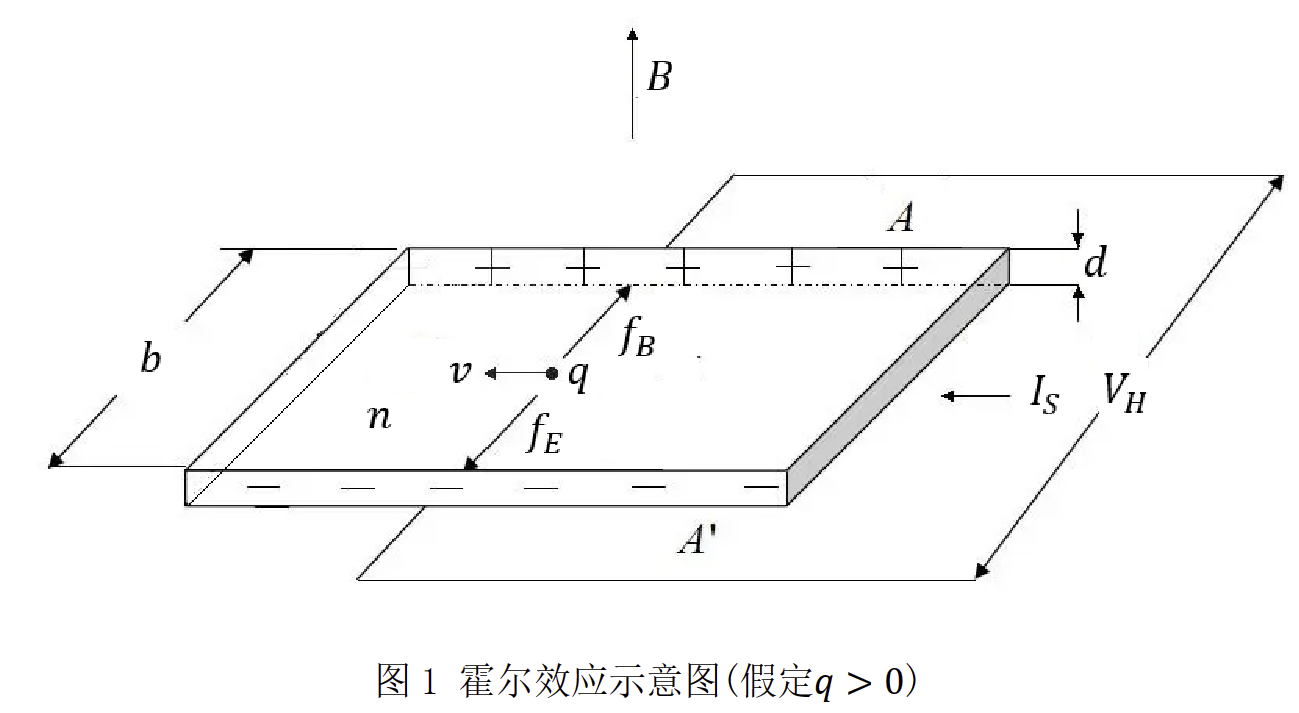
\includegraphics[width=0.7\textwidth]{hall_effect.png}
    \caption{霍尔效应示意图}
    \label{fig:hall_effect}
    \end{figure}
    
    由洛伦兹力和电场力平衡条件可得:
    
    \begin{equation}
    qvB = qE \Rightarrow E=vB
    \end{equation}
    
    而
    \begin{equation}
    V_H = Ed = vBd
    \end{equation}
    
    结合材料中电流密度 $j=qnv$,载流子速度 $v=\frac{I_S}{qnbd}$,代入上式可得:
    
    \begin{equation}
    V_H = \frac{I_SB}{qnd} \equiv K_HI_SB
    \end{equation}
    
    其中 $K_H=\frac{1}{qnd}$ 为霍尔元件的灵敏度,与材料特性有关。
    
    在实际测量中,由于制作工艺和材料非理想性,霍尔电压往往混有其他效应的贡献:
    \begin{itemize}
      \item 不等位电动势 $U_p$:电极焊接位置不同,存在与 $I_S$ 成正比的电势差
      \item 爱廷豪森效应 $U_E$:载流子速度分布不均,磁场下偏转程度不同,两侧产生温差,热电偶效应电动势正比于 $I_SB$ 
      \item 能斯特效应 $U_N$:磁场存在时,材料纵向温差会产生横向电势差,正比于 $I_S^2B$
      \item 里奇-勒杜克效应 $U_R$:磁场存在时,材料横向温差会产生纵向温差,热电偶效应电动势正比于 $I_S^2B$
    \end{itemize}
    
    霍尔元件输出电压为以上各项的叠加:
    
    \begin{equation}
    U = V_H + U_p + U_E + U_N + U_R
    \end{equation}
    
    通过改变 $I_S$ 和 $B$ 的方向,可以消除 $U_p$、$U_N$ 和 $U_R$ 的影响:
    
    \begin{equation}
    V_H + U_E = \frac{1}{4}(U_{++} - U_{+-} + U_{--} - U_{-+})  
    \end{equation}
    
    其中下标 $++$、$+-$、$--$、$-+$ 分别表示 $I_S$ 和 $B$ 同向、$I_S$ 反向 $B$ 同向、$I_S$ 和 $B$ 反向、$I_S$ 同向 $B$ 反向。在 $|V_H| \gg |U_E|$ 时,可近似得到 $V_H$。
    
    \subsection{亥姆霍兹线圈的磁场分布}
    
    亥姆霍兹线圈由两个半径为 $R$、匝数为 $N$ 的同轴环形线圈组成,两线圈平面间距为 $R$,绕组方向相同,如图\ref{fig:helmholtz_coil}所示。当通以电流 $I_M$ 时,在轴线上产生较为均匀的磁场。
    
    \begin{figure}[htbp]
    \centering
    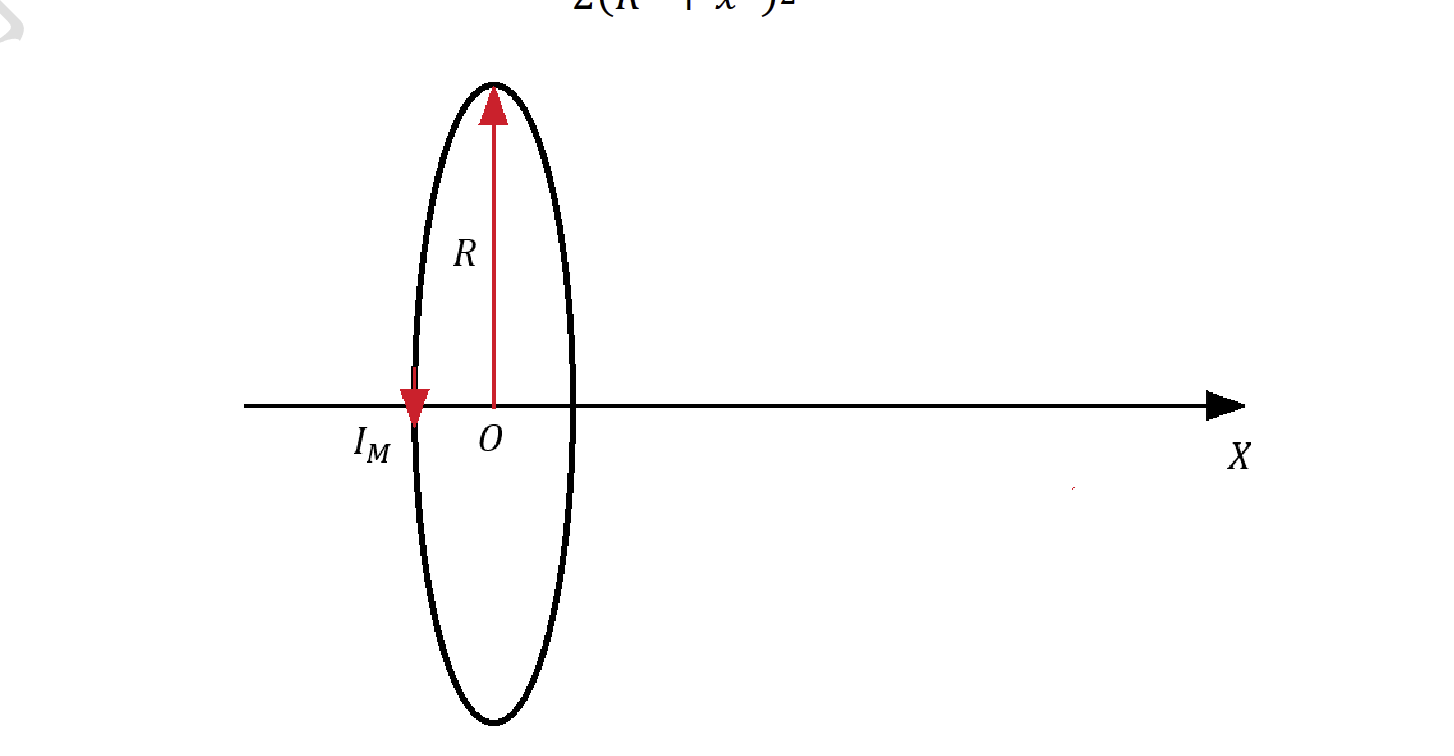
\includegraphics[width=0.7\textwidth]{helmholtz_coil.png}
    \caption{亥姆霍兹线圈示意图}
    \label{fig:helmholtz_coil}
    \end{figure}
    
    对于单个环形线圈,轴线上 $x$ 处的磁感应强度为:
    
    \begin{equation}
    B_x(x) = \frac{\mu_0 N I_M R^2}{2(R^2+x^2)^{3/2}}
    \end{equation}
    
    由磁场叠加原理,双线圈轴线上磁感应强度为:
    
    \begin{equation}
    B_x(x) = \frac{\mu_0 N I_M R^2}{2} \left[ \frac{1}{(R^2+(x+d/2)^2)^{3/2}} + \frac{1}{(R^2+(x-d/2)^2)^{3/2}} \right]
    \end{equation}
    
    可以证明,当两线圈间距等于线圈半径时,中心处 $x=0$ 满足 $\frac{\partial B_x}{\partial x}=\frac{\partial^2 B_x}{\partial x^2}=\frac{\partial^3 B_x}{\partial x^3}=0$,磁场最为均匀。
    
    \subsection{铁球在均匀磁场中的感应磁场}
    
    将一个半径为 $R$ 的铁球置于感应强度为 $\vec{B}_0=(B_0,0,0)$ 的均匀磁场中,铁球会产生感应磁化,其磁化强度 $\vec{M}$ 与外加磁场 $\vec{B}_0$ 同方向。设真空磁导率为 $\mu_0$,铁球的相对磁导率为 $\mu_r$,铁球内部感应磁场 $\vec{B}$ 满足:
    
    \begin{equation}
    \vec{B} = \mu_0(\vec{H}_0+\vec{M}) = \mu_0\left(\frac{\vec{B}_0}{\mu_0}+\frac{\mu_r-1}{\mu_r+2}\vec{B}_0\right) = \frac{3\mu_r}{\mu_r+2}\vec{B}_0 \approx 3\vec{B}_0 \quad (\mu_r \gg 1)
    \end{equation}
    
    即铁球内部磁场是外加磁场的3倍。
    
    在铁球外部,感应磁场 $\vec{B}_e$ 相当于一个磁偶极子的磁场。取铁球中心为坐标原点,z轴与外加磁场同向,则铁球表面磁荷密度 $\sigma_m=\frac{3\mu_0}{4\pi}\vec{M}\cdot\vec{e}_r=\frac{3B_0}{4\pi}\cos\theta$,其中 $\theta$ 为 $\vec{e}_r$ 与 $z$ 轴的夹角。由磁偶极子的磁位计算公式,真空中一点 $P(r,\theta)$ 处感应磁场为:
    
    \begin{equation}
        \vec{B}_e(P) = 
        \begin{cases}
            (2B_0,0,0) & r \leq R \\
            \frac{\mu_0}{4\pi}\frac{1}{r^3} \left[ \frac{3R^3B_0}{r^3}(2\cos^2\theta-\sin^2\theta)\vec{e}_r + \frac{3R^3B_0}{r^3}\sin\theta\cos\theta\vec{e}_{\theta} \right] & r > R
        \end{cases}  
    \end{equation}
    
    沿轴线 ($\theta=0$ 或 $\pi$) 方向,感应磁场与外加磁场同向,磁场加强;在赤道面 ($\theta=\pi/2$) 上,感应磁场与外加磁场反向,磁场减弱。总磁场是外加磁场与感应磁场的矢量和。


    \section{实验过程}

    \subsection{霍尔效应验证及灵敏度测量}
    
    \subsubsection{实验装置搭建}
    将两个线圈按照亥姆霍兹线圈的要求组装,并将霍尔传感器放置在线圈中心。调节电源输出,左路恒流源为线圈提供励磁电流 $I_M$,右路恒流源为霍尔元件提供工作电流 $I_S$。用万用表分别检查 $I_M$ 和 $I_S$ 是否达到设定值。
    
    \subsubsection{霍尔电压与磁场关系测量}
    固定 $I_S=10mA$,改变 $I_M$ 从 $0\sim1000mA$,每隔 $100mA$ 记录对应的 $B$ 和 $V_H$。由于
    \begin{equation}
        B_{center}(I_M) = \frac{\mu_0 N I_M R^2}{(R^2+(d/2)^2)^{3/2}} 
        \end{equation}
    $I_M$ 和 $B$ 成正比,改变 $I_M$ 即可得到不同的 $B_{center}$ 值。
    
    在每个 $I_M$ 下,需要测量 4 种 $I_S$ 和 $I_M$ 组合下的霍尔电压,然后按照
    \begin{equation}
    V_H = \frac{1}{4}(U_{++} - U_{+-} + U_{--} - U_{-+})
    \end{equation} 
    计算 $V_H$,消除其他效应的影响。
    
    数据记录完毕后,以 $B$ 为横轴,$V_H$ 为纵轴作图。根据理论分析,两者应呈线性关系:
    \begin{equation}
    V_H = K_H I_S B_{center}
    \end{equation}
    用最小二乘法拟合直线,斜率即为灵敏度 $K_H$。
    

    
    \subsubsection{霍尔电压与工作电流关系测量}
    固定 $I_M=1000mA$,改变 $I_S$ 从 $0\sim10mA$,每隔 $1mA$ 记录对应的 $I_S$ 和 $V_H$。测量步骤与数据处理方法同上。
    
    作 $V_H-I_S$ 图,两者应呈线性关系,斜率为 $K_H B$。结合已知的 $B$ 值,可再次计算 $K_H$,并与上一小节的结果对比,验证实验的重复性。
    

    
    \subsection{亥姆霍兹线圈磁场分布测量}
    \subsubsection{建立 $V_H-U_{++}$ 关系}
    根据上一节的测量结果,建立 $V_H$ 与 $U_{++}$ 的对应关系。可采用线性拟合:
    \begin{equation}
    V_H = k U_{++} + b    
    \end{equation}
    或多项式拟合:
    \begin{equation}
    V_H = a_0 + a_1 U_{++} + a_2 U_{++}^2 + \cdots + a_n U_{++}^n    
    \end{equation}
    选择拟合优度高的模型,后续只需测量 $U_{++}$ 即可间接得到 $V_H$ 和 $B$。
    
    \subsubsection{磁场分布测量}
    固定 $I_M=1000mA$,沿线圈轴线方向移动霍尔传感器,每隔 $1cm$ 测量 $U_{++}$,并换算为 $B$。以轴线坐标 $x$ 为横轴,$B$ 为纵轴作图,得到磁场分布曲线。
    
    \begin{figure}[htbp]
    \centering
    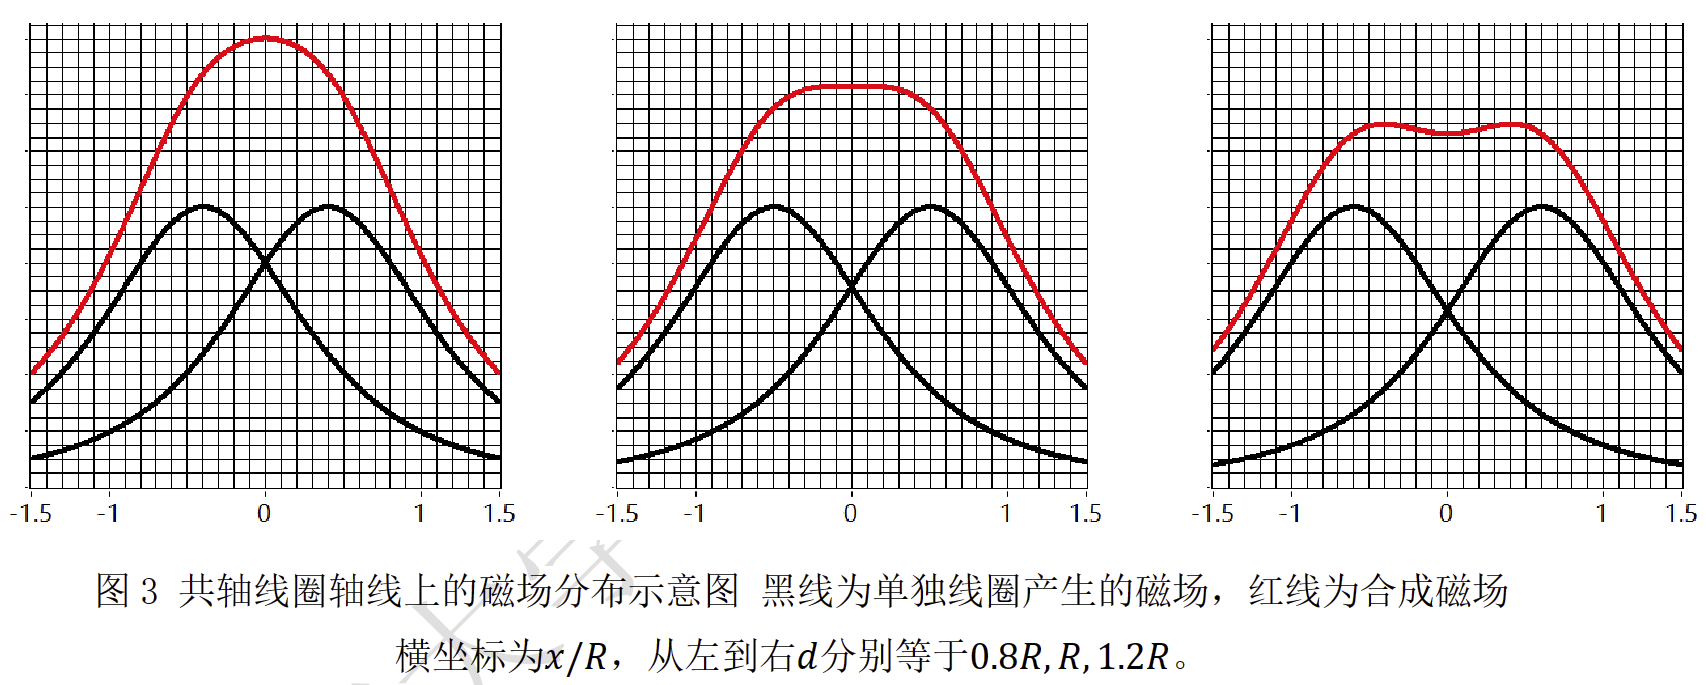
\includegraphics[width=0.6\textwidth]{B-x.png}
    \caption{亥姆霍兹线圈轴线上磁场分布(示意图)}
    \label{fig:B-x}
    \end{figure}
\newpage
    从曲线上找出磁场最大值 $B_{max}$,分别计算 $0.95B_{max}$、$0.9B_{max}$ 和 $0.8B_{max}$ 对应的 $x$ 坐标范围,即磁场均匀度不同的区域大小。
    
    \subsection{铁球感应磁场测量}
    将铁球置于亥姆霍兹线圈中心,调节 $I_M=1000mA$,测量轴线上不同位置的磁感应强度 $B_{total}$。由于
    \begin{equation}
    \vec{B}_{total} = \vec{B}_0 + \vec{B}_e     
    \end{equation}
    为了得到铁球的感应磁场 $\vec{B}_e$,需要扣除外加磁场 $\vec{B}_0$。
    
    将测量结果与理论计算公式对比:
    \begin{equation}
    \vec{B}_e(x) = \frac{2R^3 B_0}{x^3}\vec{e}_x \quad (x > R)
    \end{equation}
    其中 $R$ 为铁球半径,$x$ 为距离铁球中心的距离。
    
    
    比较实验结果与理论预期,分析误差来源。
    
    \subsection{其他测量(可选)}
    可以探究铁球尺寸、材料、外加磁场强度等因素对感应磁场的影响。
    
    以上是实验过程的详细描述,包括实验装置搭建、测量步骤、数据记录与处理、结果分析等。通过测量霍尔电压与磁场、工作电流的关系,验证霍尔效应的理论公式,并计算灵敏度。通过测量亥姆霍兹线圈轴线上的磁场分布,分析磁场的均匀性。通过测量铁球在均匀磁场中的感应磁场,并与理论计算结果对比,加深对磁介质磁化过程的理解。
    
    在实验过程中需要注意以下事项:
    \begin{itemize}
        \item 霍尔电压较小,读数时避免外界电磁干扰,做好屏蔽措施
        \item 改变 $I_S$ 和 $I_M$ 方向时动作要轻,避免线圈和传感器移位
        \item 测量磁场分布时,每次移动传感器后让读数稳定再记录
        \item 铁球表面应洁净,感应磁场测量前先退磁
    \end{itemize}

    \section{预习思考题}

\subsection{根据霍尔效应能否确定材料中载流子带的是正电荷还是负电荷?}
根据霍尔效应能确定载流子电荷的符号,从而确定其是正电荷还是负电荷。
由公式:
    \begin{equation}
    V_H = \frac{I_SB}{qnd} \equiv K_HI_SB
    \end{equation}
可见,不同电荷的载流子在相同条件下,霍尔电压的符号相反。因此,通过测量霍尔电压的正负号,可以确定载流子的电荷是正电荷还是负电荷。
\subsection{不等位电动势能否单独测量?}
不等位电动势 $U_p$ 可以单独测量,因为$U_p$是所有附加电动势和霍尔电动势中唯一与磁场无关的的,只要做好磁屏蔽,就能直接测量不等位电动势。

\subsection{如何尽量准确地把传感器放到亥姆霍兹线圈的对称中心点?}
可以利用磁场分布的对称性,通过以下步骤找到亥姆霍兹线圈的中心点:
\begin{enumerate}
    \item 先将传感器大致放在两线圈的中间位置,调节 $I_M$ 至较大值,记录此时的霍尔电压 $V_H^0$,左右移动霍尔传感器,分辨此时中间位置为局部极强还是极弱。
    \item 沿轴线方向略微移动传感器,记录 $V_H$ 的变化。如果 $V_H$ 增大,则向 $V_H$ 增大(减小)的方向移动;如果 $V_H$ 减小,则向相反方向移动。
    \item 重复步骤2,直到找到 $V_H$ 局部极强或极弱的位置,该位置即为也就是线圈中心。
    \item 在中心附近的小范围内多次测量,取 $V_H$ 最大时传感器的位置,以进一步提高精度。
\end{enumerate}

之所以 $V_H$ 最大处为线圈中心,是因为亥姆霍兹线圈的磁场分布在中心处取局部极值,且沿轴线方向对称。设中心处磁感应强度为 $B_0$,则轴线上任一点的磁感应强度为:
\begin{equation}
B(x) = B_0 \left[ \frac{1}{(1+x'^2)^{3/2}} + \frac{1}{(1+x'^2)^{3/2}} \right], \quad x' = \frac{2x}{R}
\end{equation}
其中 $x$ 为距中心的距离,$R$ 为线圈半径。函数 $B(x)$ 在 $x=0$ 处取得极值。

\subsection{如何测量铁球的感应磁场?}
测量铁球的感应磁场,需要先测量外加均匀磁场 $\vec{B}_0$,再测量铁球置于磁场中时的总磁场 $\vec{B}_{total}$,两者相减即为铁球的感应磁场 $\vec{B}_e$:
\begin{equation}
\vec{B}_e = \vec{B}_{total} - \vec{B}_0
\end{equation}

具体步骤如下:
\begin{enumerate}
    \item 先不放铁球,只用亥姆霍兹线圈产生均匀磁场,测量不同位置的 $\vec{B}_0$。
    \item 将铁球置于线圈中心,测量不同位置的 $\vec{B}_{total}$,注意传感器不要碰到铁球。
    \item 根据位置对应相减,得到铁球在不同位置产生的感应磁场 $\vec{B}_e$。
    \item 将测量结果与理论公式对比:
    \begin{equation}
    \vec{B}_e(r,\theta) = 
    \begin{cases}
        \frac{2\mu_0}{3}\vec{B}_0 & r < R \\
        \frac{\mu_0}{4\pi}\frac{R^3}{r^3} \left[ (2\cos^2\theta-\sin^2\theta)\vec{e}_r + \sin\theta\cos\theta\vec{e}_{\theta} \right]B_0 & r > R
    \end{cases}
    \end{equation}
\end{enumerate}

其中 $R$ 为铁球半径,$r$、$\theta$ 为极坐标系下铁球中心到测量点的距离和天顶角,$\vec{e}_r$ 和 $\vec{e}_{\theta}$ 为单位径向矢量和单位角向矢量。

\subsection{磁场中两个铁球的感应磁场是否具有可加性?为什么?}
两个铁球的感应磁场不具有可加性,即两个铁球同时置于磁场中产生的感应磁场,不等于它们分别置于磁场中产生的感应磁场之和。这是因为每个铁球磁化时,除了外加磁场 $\vec{B}_0$ 之外,还受到另一个铁球感应磁场的影响。
。
\end{document}
